\chapter{结果分析}\thispagestyle{fancy}
本章主要对三个模型的准确率和时空复杂度进行测评,此外,本章对神经网络模型中的各项参数进行了分析。
\section{模型分析} \label{sec:modeleval}
\subsection{实验条件}
为了证实文本提出的知识模型,NOLSTM模型和CLSTM模型的有效性,本章使用NLPCC 2014的SCDL数据集和用于展示的携程数据集进行测评,实验条件如下:\par
运行参数:\par
\begin{itemize}
\item 操作系统: ubuntu16.10 64位
\item 运行平台: tensorflow v1.1
\item 磁盘空间: 1.9 TB
\item 内存空间: 32 GB
\item 处理器: Intel Core i7-6700 3.40 GHz x 8
\end{itemize}
\par 
神经网络参数:


\begin{center}
\begin{longtabu} to \textwidth{X|X|X|X}
\hline
参数名称 & 模型 & 数据集 & 参数值
\\\hline
离散特征编码长度 & - & CLSTM和NOLSTM & 32
\\\hline
稀有词限定最低频度 & NLPCC2014SCDL中文数据集 & CLSTM,NOLSTM & 'all': 7, 'nt': 12, 'ns': 12, 'nrf':12, 'nto': 12, 'null': 12, None: 12
\\\hline
稀有词限定最低频度 & NLPCC2014SCDL中文数据集 & CLSTM,NOLSTM & 'all': 7
\\\hline
稀有词限定最低频度 & 携程数据集 & CLSTM,NOLSTM & 'all': 7
\\\hline
batch大小 & - & CLSTM和NOLSTM & 200句
\\\hline
步数 & - & CLSTM & 10
\\\hline
每步包含词数 & NLPCC2014SCDL中文数据集 & CLSTM & 50
\\\hline
每步包含词数 & NLPCC2014SCDL英文数据集 & CLSTM & 250
\\\hline
每步包含词数 & 携程数据集 & CLSTM & 50
\\\hline
词数 & NLPCC2014SCDL中文数据集 & NOLSTM & 200
\\\hline
词数 & NLPCC2014SCDL英文数据集 & NOLSTM & 1000
\\\hline
词数 & 携程数据集 & NOLSTM & 250
\\\hline
LSTM单元维度 & - & CLSTM & 256
\\\hline
线性层0维度 & - & NOLSTM & 512
\\\hline
线性层1维度 & - & CLSTM,NOLSTM & 256
\\\hline
线性层2维度 & - & CLSTM,NOLSTM & 64
\\\hline
初始学习速率 & - & CLSTM & 1.0
\\\hline
初始学习速率 & - & NOLSTM & 0.1
\\\hline
Dropout Keep Rate & - & CLSTM,NOLSTM & 0.6
\\\hline
验证间隔 & NLPCC2014SCDL & CLSTM,NOLSTM & 40步 
\\\hline
验证间隔 & 携程数据集 & CLSTM,NOLSTM & 200步
\\\hline
\end{longtabu}
\end{center}

\subsection{精度分析}
本文中验证标准为准确率,即分类正确的语句占测试集的百分比。\par
神经网络模型的测试方法为:\par
\begin{itemize}
\item NLPCC 2014的SCDL数据集在官方训练集上进行封闭训练,使用官方测试集作为测试集。
\item 携程数据集使用5-fold进行测试,依次选取其中一个子集作为验证集,一个子集作为测试集,最终的测试准确率为五次平均。
\end{itemize}


准确度结果如下表:
\begin{center}
\begin{longtabu} to \textwidth{X|X|X|X|X}
\hline
数据集名称 & 知识模型 & CNNPL & CNNLSTMPL & NLPCC-best
\\\hline
携程数据集 & 69.9\% & 74.3\% & 76.7\% & -
\\\hline
NLPCC 2014 SCDL 中文 & 69.7\% & 76.3\% & 77.5\% & 76.9\%
\\\hline
NLPCC 2014 SCDL 英文 & 76.2\% & 85.2\% & 86.3\% & 86.0\%
\\\hline
\end{longtabu}
\end{center}


其中NLPCC-best为官方正式比赛中最高的准确率\cite{nlpccres},这里由于NLPCC测试集中正向:负向为1:1,所以该准确率为$\frac{NP + PP}{2}$。\par
从表中可以得出,CLSTM和NOLSTM在数据集上的表现都较好,接近或略高于第一名的准确度,知识模型的表现略差。由此可以证明CLSTM和NOLSTM模型是有效的,而知识模型还需要再加以改进。同时,CLSTM模型的精度往往高于NOLSTM模型,这可能是由于CLSTM模型一次处理的单词较少,从而需要训练的参数更少,而且CLSTM模型更能利用自然语言的序列信息。综合来看,基于深度学习的神经网络不需要大量语言学知识,也不依赖于情感词典和语法分析工具,却可以通过学习特征表达的方式达到超过传统的基于知识的模型的性能。\par

\subsection{时空复杂度分析}
时间消耗如下表(取到达最高精度的时间):\par
\begin{center}
\begin{longtabu} to \textwidth{X|X|X|X} 
\hline
数据集名称 & 知识模型 & NOLSTM & CLSTM
\\\hline
携程数据集 & 18770s & 1921s & 5350s % 
\\\hline
NLPCC2014SCDL中文 & 2768s & 564s & 1366s % 
\\\hline
NLPCC2014SCDL英文 & 3125s & 1389s & 3138s % 
\\\hline
\end{longtabu}
\end{center}
\par
由于CLSTM模型需要反复迭代,因此CLSTM模型速度较LSTM模型更差,由于训练策略的原因,CLSTM模型并不特意将长度相似的语句放在同一个batch中,这导致短句处理完毕后模型需要接受短句的补零,如果长句均匀分布在训练集内,就会导致训练速度下降。\par
知识模型速度较慢的原因可能有四点:1. 知识模型启动时需要同时启动ansj和stanfordParser的中英版本,耗时较多。2. 知识模型在实现中不直接使用分词后的词语,而是主动调用分词工具,因此导致时间较慢。 3. 知识模型需要对每条语句建立语法树,因此耗时较多。 4. 知识模型通过jpype调用java实现,中间操作较多,且jpype需要管理和启动java虚拟机。\par
\begin{center}
\begin{longtabu} to \textwidth{X|X|X|X}
\hline
数据集名称 & 知识模型 & NOLSTM & CLSTM \\
\hline
NLPCC2014SCDL中文 & 12276572K & 3733108K & 5905060K \\
\hline
NLPCC2014SCDL英文 & 12276572K & 3408696K & 5686756K
\\\hline
\end{longtabu}
\end{center}


从表中可以总结出在三种模型中NOLSTM的速度最快,空间消耗率是最低的,因此,可以得出结论,在文本较短情感较为强烈时,使用NOLSTM模型是节约时间和空间的做法,而如果需要处理不定长的文本,或者对精度要求较高,则应当使用CLSTM模型。\par
\section{参数分析}
本节分析对比神经网络模型的各种基本参数以及策略,由于神经网络训练较为费时,所以本节选取NOLSTM模型,使用NLPCC2014SCDL中文数据集进行训练,以对比不同参数或策略条件下的精度,得出最优参数或策略。
\subsection{初始编码策略}
在预处理过程中,本文使用word2vec训练待编码的离散特征向量。为了探究该步骤是否存在意义,本文使用NOLSTM模型,在参数相同的情况下分别运行了三次,第一次使用word2vec初始化编码,第二次使用零矩阵初始化编码,第三次则使用截断的正态分布随机初始化向量,取mean=0,stddev=0.1,准确率随训练过程的变化如图\ref{femb}:


通过观察该图内的三条曲线,可以发现word2vec的编码准确率较高,正态分布的编码准确率次之,但也呈现上升趋势,并且随时间逐渐接近word2vec编码的准确率,而零矩阵则无法训练,几乎保持为一条直线。综上所述,可以认为word2vec编码加快了训练速度,并且可能提高模型准确率。因此,使用word2vec初始化编码是有意义的。
\begin{center}
\begin{figure}[!hbp]
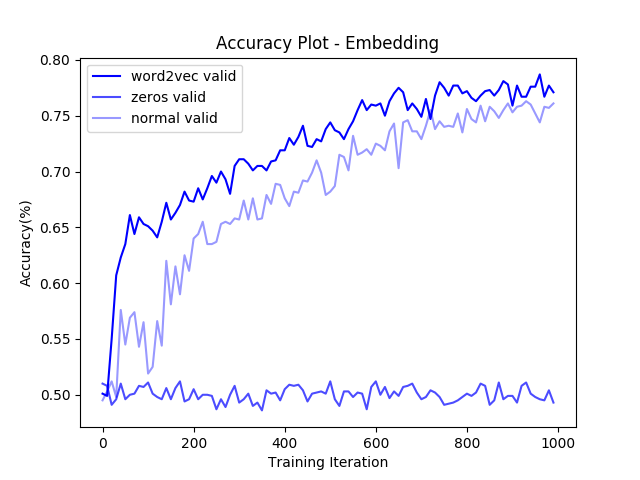
\includegraphics[width=0.8\textwidth]{graphic/emb.png}
\caption{编码-准确率变化图 \label{femb}}
\end{figure}
\end{center}
\subsection{优化函数选择}
本文中NOLSTM模型和CLSTM模型都使用ADAM算法作为优化函数。本小节中对本文中使用的优化函数做出评估,分别使用SGD算法,ADADELTA算法和ADAM算法在同样的参数下各自训练NOLSTM模型,得到准确率随时间的变化曲线如图\ref{fopt}:


通过观察图中的三条曲线,可以发现ADAM的训练速度和准确率都最高,SGD次之,而ADADELTA最慢。实际上,这是因为ADADELTA算法陷入了局部最小值点。综上所述,可以认为选择ADAM作为优化函数是正确的。实际上,SGD算法也是学术研究中较为常用的算法,如果人工配置的学习率足够强大,往往能够得到自适应梯度的优化函数所不能得到的效果。
\begin{center}
\begin{figure}[!hbp]
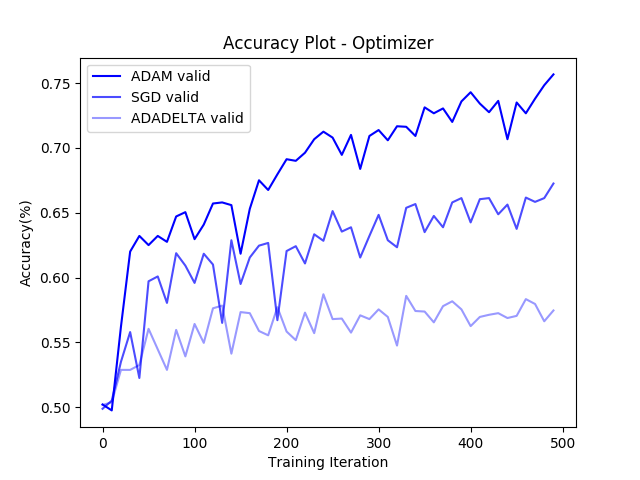
\includegraphics[width=0.8\textwidth]{graphic/opt.png}
\caption{优化函数-准确率变化图 \label{fopt}}
\end{figure}
\end{center}
\subsection{激活函数选择}
本文中模型都使用ReLU算法作为线性层之间的激活函数。本小节中对本文中使用的激活函数做出评估,分别使用ReLU算法,tanh算法和sigmoid算法在同样的参数下各自作为线性层之间的激活函数训练NOLSTM模型,得到准确率随时间的变化曲线如图\ref{fnonlinear}:


在训练过程中,三种函数所对应的模型都保持近似于一致的上升趋势,但当训练进入后期,接近最高准确率时,ReLU也即颜色最深的曲线的准确率保持最高,因此,可以认为ReLU相较于sigmoid函数和tanh函数来说更适宜作为线性层之间的激活函数。这可能与ReLU具有单侧抑制和稀疏激活性有关。
\begin{center}
\begin{figure}[!hbp]
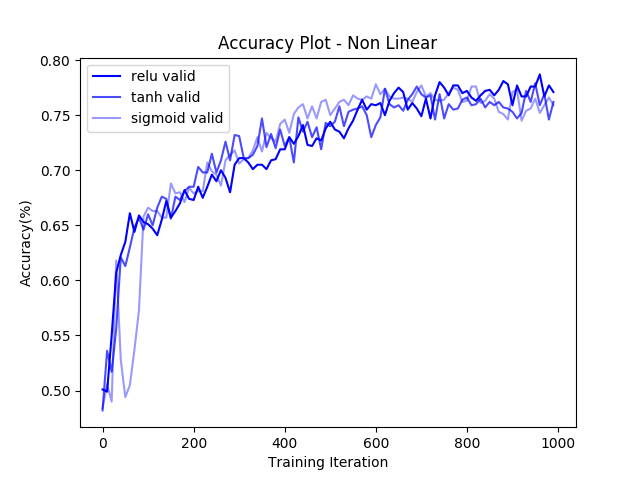
\includegraphics[width=0.8\textwidth]{graphic/nonlinear.png}
\caption{激活函数-准确率变化图 \label{fnonlinear}}
\end{figure}
\end{center}
\subsection{是否过滤稀有词} \label{sec:rareword}
本文在预处理过程中会对离散特征做过滤稀有词操作,即按照词性和最低频度将频度小于此词性的最低频度的离散特征转化为一个特殊的词,"RAREWORD"。本小节探讨该操作的必要性。


如图\ref{frareword},明显,使用全部单词,不进行稀有词过滤的模型准确率较低,泛化性能较差。从另一方面来说,例如数据集中只有一条负向文本中出现了"北京饭店"这个稀有词汇,则神经网络极有可能将"北京饭店"学习为负向情感词汇,但实际上该词汇是中性的实体词汇。通过过滤稀有词,模型能够尽力保证词汇在多种句式中出现,从而能够学习到词汇的真正含义,避免被标注影响,也能帮助抽取高级特征。
\begin{center}
\begin{figure}[!hbp]
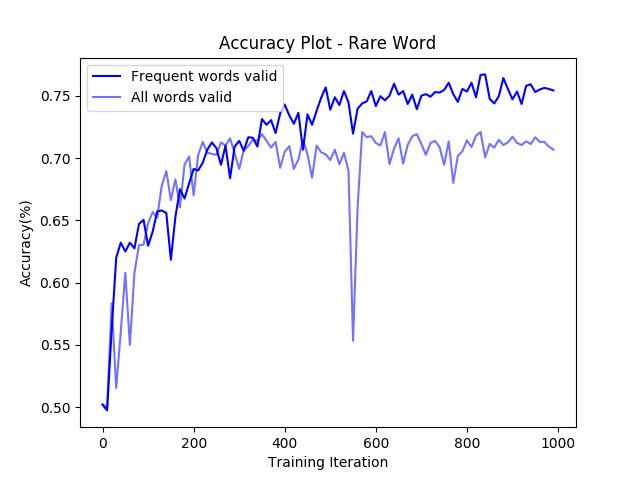
\includegraphics[width=0.8\textwidth]{graphic/rareword.png}
\caption{是否过滤稀有词-准确率变化图 \label{frareword}}
\end{figure}
\end{center}
\subsection{是否使用dropout}
dropout函数随机使输出单元的一部分为0,即使其输出无效。使用dropout函数往往能够迫使模型学习更加健壮的特征,避免被局部特征所误导,可以减轻局部最小值的问题。但dropout本身可能导致模型精度无法提升等问题。本小节讨论神经网络模型在处理情感分类任务中dropout是否必要。如图\ref{fdropout},分别进行了两次训练,一次dropout 保持不变的可能性设置为0.6,另一次不设置dropout。


从图中可以看出,尽管在训练的早期阶段无dropout的模型准确率上升速度更加快,但在后期使用dropout的算法能明显增加准确度。因此,可以认为使用dropout不仅能影响到准确率,而且还是必要的,能够帮助泛化。在实践中,为了体现dropout的效果,本文将之设为0.6。
\begin{center}
\begin{figure}[!hdp]
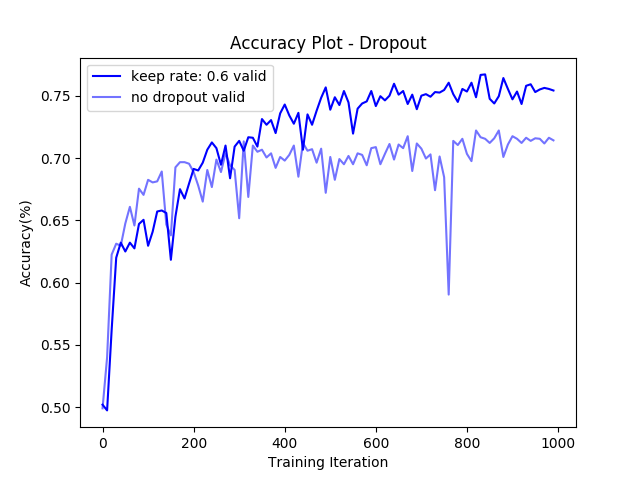
\includegraphics[width=0.8\textwidth]{graphic/dropout.png}
\caption{有无Dropout-准确率变化图 \label{fdropout}}
\end{figure}
\end{center}
\subsection{卷积核研究}
实际上,在没有接触到NLPCC2014的任务集之前,笔者认为局部池化,尤其是堆叠卷积网络加池化的能够抽取出高级的语法特征,更适应于情感分类任务,但实际上,在本文所做过的测试中,核较小的卷积加全局池化的性能往往优于堆叠卷积网络加池化。


本小节使用一种特殊的方法表示卷积核,【3,4,5,6,7】(【-1,-1,-1,-1,-1】)代表只有一维卷积,分别是核大小为3,4,5,6,7的的卷积,每个卷积输出使用全局池化处理,【2,3,5】(【2,3,5】)代表只有一维卷积,分别是核为2,步长为1的,由大小为2,步长为2的最大池化层处理的卷积输出,核为3,步长为1的,使用大小为3,步长为3的最大池化进行处理的卷积输出和核与池化层,步长都为5的卷积输出。【2,3,5】(【2,3,5】),【1,2,3】(【1,2,3】)则代表在【2,3,5】(【2,3,5】)输出的特征上,分别做卷积核大小为1,2,3,池化层大小和步长对应为1,2,3的卷积->池化操作。


本文进行了一系列实验,相关准确度如下:


\begin{itemize}
\item 【3,5,6,7,9】 (【-1,-1,-1,-1,-1】): 0.75
\item 【3,5,7,9】(【-1,-1,-1,-1】):0.73
\item 【1】(【1】): 0.66
\item 【2,3】(【2,3】),【3,5,6,7,9】 (【-1,-1,-1,-1,-1】):0.71
\item 【2,3,5】(【2,3,5】),【1,2,3】(【2,3,5】),【1,2,3】(【2,3,5】):0.75
\item 【3,5,7】(【3,5,7】),【1,2,3】(【2,3,5】),【1,2,3】(【2,3,5】):0.73
\item 【2,3,5】(【2,3,5】),【1,2,3】(【1,2,3】): 0.68
\item 【2,2,2,2】(【2,2,2,2】): 0.56
\item 【2,2,2,2】(【2,2,2,-1】): 0.55
\item 【2,3,4】: 0.63
\item 【3,4,5】: 0.64
\item 【4,5,6】: 0.54
\item 【2,3,4】(【2,3,4】): 0.62
\item 【3,4,5】(【3,4,5】)
\item 【9,11,13】(【-1,-1,-1】): 0.68
\item 【2,3,5】(【-1,-1,-1】): 0.65
\item ...
\end{itemize}

在实验中,可以发现堆叠卷积神经网络并不能改进模型性能。综合考虑后,模型决定采用【3,5,6,7,8】(【-1,-1,-1,-1,-1】),因为它不仅精度最高,而且表现更为稳定,训练速度也较快。当卷积核为1,池化层也为1时,模型相当于LSTM模型,在实践中,该模型效果不佳,不能泛化出应有结果。

